\documentclass[a4paper,fleqn,bahasa]{article}

\usepackage{babel}

\usepackage[a4paper]{geometry}
\usepackage{NotesTeX}
%\geometry{verbose,tmargin=2.5cm,bmargin=2.5cm,lmargin=2.5cm,rmargin=2.5cm}

\setlength{\parskip}{\smallskipamount}
\setlength{\parindent}{0pt}

\usepackage{amsmath}
\usepackage{amssymb}
\usepackage{braket}

\usepackage[libertine]{newtxmath}
\usepackage[no-math]{fontspec}
\setmainfont{Linux Libertine O}
%\setmonofont{JuliaMono-Regular}

\usepackage{hyperref}
\usepackage{url}
\usepackage{xcolor}

\usepackage[normalem]{ulem}

\usepackage{mhchem}

\usepackage{minted}
\newminted{text}{breaklines,fontsize=\footnotesize}
\newminted{dart}{breaklines,fontsize=\footnotesize}

\newcommand{\txtinline}[1]{\mintinline[fontsize=\normalsize]{text}{#1}}

\definecolor{mintedbg}{rgb}{0.90,0.90,0.90}
\usepackage{mdframed}

%\BeforeBeginEnvironment{minted}{\begin{mdframed}[backgroundcolor=mintedbg,%
%  rightline=false,leftline=false,topline=false,bottomline=false]}
%\AfterEndEnvironment{minted}{\end{mdframed}}

\usepackage{tikz}
\usetikzlibrary{shapes.geometric}
\tikzstyle{mybox} = [draw=blue, fill=green!5, very thick, rectangle,
  rounded corners, inner sep=10pt, inner ysep=20pt]
\tikzstyle{fancytitle} = [fill=blue, text=white]

\begin{document}

\title{
  \begin{center}{
    \Huge \textit{Latihan Flutter}}\\
    {{\itshape MI3103}}
\end{center}
}
\author{Fadjar Fathurrahman}


\affiliation{
Program Studi Teknik Fisika \\
Fakultas Teknologi Industri \\
Institut Teknologi Bandung
}

\emailAdd{fadjar.fathurrahman@gmail.com}
\emailAdd{fadjar@tf.itb.ac.id}

%\title{\textsf{PWDFT.jl} Documentation}
%\author{Fadjar Fathurrahman}
%\date{}

\maketitle

\newpage

\part{MaterialApp}

\section{Struktur program}

Berikut ini adalah struktur program sederhana yang akan digunakan
\begin{dartcode}
import 'package:flutter/material.dart';
  
void main() => runApp(MyApp());
  
class MyApp extends StatelessWidget {
  @override
  Widget build(BuildContext context) {
    return MaterialApp(
      title: 'Flutter Demo',
      theme: ThemeData(
        primarySwatch: Colors.blue,
      ),
      home: MyHome(),
    );
  }
}
  
class MyHome extends StatelessWidget {
  @override
  Widget build(BuildContext context) {
    return Scaffold(
      appBar: AppBar(
        title: Text('MyHome')
      ),
      body: Center(
        child: Text('This is my home'),
      ),
    );
  }
}
\end{dartcode}

Tampilan dari program ini dapat dilihat pada Gambar \ref{fig:MyHome-debug}.
\begin{marginfigure}
{\centering
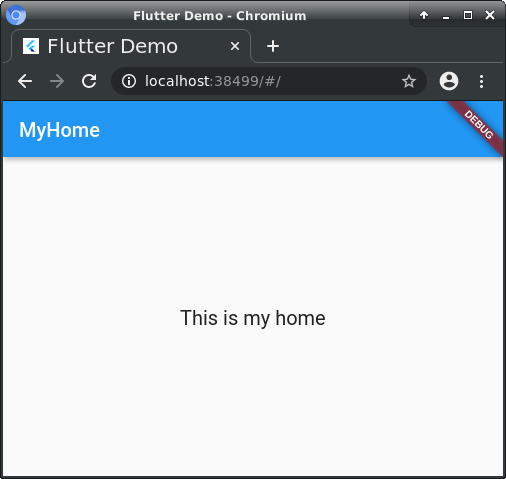
\includegraphics[width=\marginparwidth]{images/MyHome_debug.png}
\par}
\caption{Tampilan MyHome.}
\label{fig:MyHome-debug}
\end{marginfigure}

\section{Menghilangkan banner debug}

Banner debug pada tampilan aplikasi dapat dihilangkan dengan
mengatur parameter \\
\txtinline{debugShowCheckedModeBanner} menjadi \txtinline{false}.

Contoh:
\begin{dartcode}
class MyApp extends StatelessWidget {
  @override
  Widget build(BuildContext context) {
    return MaterialApp(
      title: 'Flutter Demo',
      theme: ThemeData(
        primarySwatch: Colors.blue,
      ),
      home: MyHome(),
      debugShowCheckedModeBanner: false,
    );
  }
}
\end{dartcode}

\begin{marginfigure}
{\centering
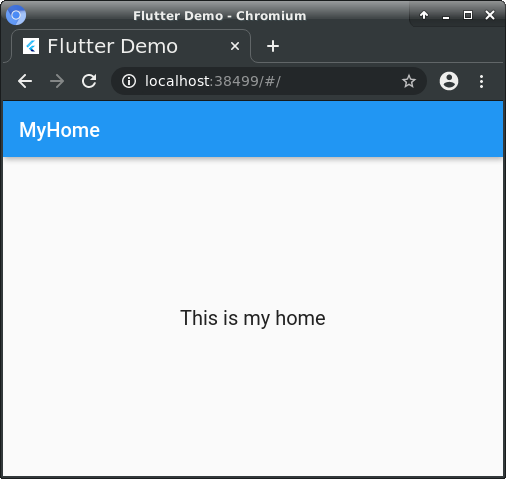
\includegraphics[width=\marginparwidth]{images/MyHome_01.png}
\par}
\caption{Tampilan MyHome tanpa banner debug.}
\end{marginfigure}


\bibliographystyle{unsrt}
\bibliography{BIBLIO}



\end{document}
